%%%%%%%%%%%%%%%%%%%%%%%%%%%%%%%%%%%%%%%%%%%%%%%%%%%%%%%%%%%%%%%%%%%%%
%%DEFINITIONS
\def\+{+}
\def\.{\cdot}
\def\~#1{\overline{#1}}
\def\<#1>{\langle#1\rangle}
%%%%EXERCISE
\count32=0
\def\exercise{\global\advance\count32 by1
{\medskip\noindent\bf Exercício \the\count32.~}}
%%%%AXIOM
\count31=0
\def\axiom#1{\global\advance\count31 by1%
{\medskip\noindent\bf Axioma~\the\count31.~}}
%%%%THEOREM
\count30=0
\def\theorem#1{\global\advance\count30 by1%
{\medskip\noindent\bf Teorema \the\count30.~}}
%%%%PROOF
\def\proof{\smallskip\noindent{\it Prova.\/}}
%%%%
%\newtheorem{theorem}{Teorema}[section]
%\newtheorem{lemma}[theorem]{Lema}
%\newtheorem{proposition}[theorem]{Proposição}
%\newtheorem{corollary}[theorem]{Corolário}
%\newenvironment{proof}[1][Prova]{\begin{trivlist}
%\item[\hskip \labelsep {\bfseries #1}]}{\end{trivlist}}
\newenvironment{definition}[1][Definição]{\begin{trivlist}
\item[\hskip \labelsep {\bfseries #1}]}{\end{trivlist}}
\newenvironment{example}[1][Examplo]{\begin{trivlist}
\item[\hskip \labelsep {\bfseries #1}]}{\end{trivlist}}
\newenvironment{remark}[1][Remark]{\begin{trivlist}
\item[\hskip \labelsep {\bfseries #1}]}{\end{trivlist}}
\newcommand{\qed}{\nobreak \ifvmode \relax \else
      \ifdim\lastskip<1.5em \hskip-\lastskip
      \hskip1.5em plus0em minus0.5em \fi \nobreak
      \vrule height0.75em width0.5em depth0.25em\fi}
%%%%%%%%%%%%%%%%%%%%%%%%%%%%%%%%%%%%%%%%%%%%%%%%%%%%%%%%%%%%%%%%%%%%%

\paragraph{Introdução.}
A {\it Álgebra} é o ramo da matemática em que símbolos são usados para
representar números ou quantidades em fórmulas e equações. Por
exemplo, as seguintes equações

$$ax + b =0,$$
$$ax^2 + bx + c = 0,$$
$$ax^3 + bx^2 + cx + d = 0,$$

\noindent provenientes da Álgebra Elementar ou Convencional, possuem
solução exata e podem ser utilizadas para resolver diversos
problemas. A palavra ``Álgebra'' -- {\it al jebr} em arábico -- foi
primeiro usada por Mohammed of Kharizm que ensinava matemática em
Bagdá no século IV, e significa reunião de partes quebradas.

Os sistemas matemáticos atuais são construídos a partir de {\bf
  axiomas}, que são equações simples e fundamentais que não podem ou
precisam ser provadas. O sistema axiomático teve como precursor o
livro ``Os Elementos'' ($\sim300$A.C.) do matemático Euclides que
formulava 465 propriedades (teoremas) geométricas a partir de
postulados (axiomas).  Como exemplo, a seguinte premissa foi extraída
do livro:

\begin{quote}
``Uma linha reta pode ser desenhada entre quaisquer dois pontos.''
\end{quote}

Euclides postulou que as propriedades de um ponto não precisam ser
demonstradas por serem instrísecas. Fora os axiomas, todas as demais
propriedades (teoremas) devem ser provadas.

Os matemáticos descobriram que qualquer sistema formal pode ser
construído a partir de alguns poucos axiomas, tais como, a Teoria das
Probabilidades, Geometria, Álgebra, dentre outros.

Como exemplo de construção de um sistema axiomático poderíamos ter as
seguintes leis de um conjunto $A$, que permite as operações $\circ$ e
$\triangle$.

\begin{enumerate}
\item Comutativa: $x\triangle y=y\triangle x$;
\item Associativa: $x\triangle (y\triangle z)= (x\triangle y)\triangle z$;
\item Distributiva: $x\triangle (y\circ z) = (x\triangle y)\circ (x\triangle z)$,\quad
  $x\circ (y\triangle z) = (x\circ y)\triangle (x\circ z)$;
\item Identidade (Elemento neutro $e$): $e\triangle x=x\triangle e=x$.
\end{enumerate}

A abstração e generalização destes sistemas permite a substituição dos
símbolos por conceitos de uma área específica que satisfaçam os
axiomas, sem a necessidade de se construir um novo sistema formal para
cada nova área do conhecimento.

\section{Álgebra Booleana}

Os fundamentos da Álgebra Booleana foram descritos no livro ``An
Investigation of the Laws of Thought'' de George Boole, publicado em
1854~\cite{boole1854}. Sua primeira aplicação conhecida foi proposta
por Shannon para modelar circuitos comutadores telefônicos baseados em
relés~\cite{shannon1937}.

\paragraph{Definições.}
Considere um tupla

$$\<B,\+,\.,0,1>$$

\noindent em que $B$ é um conjunto, $\+$ e $\.$ são operações binárias
em $B$; $0$ e $1$ são membros distintos de $B$. O sistema algébrico
assim definido é uma {\bf Álgebra Booleana} se satisfizer os seguintes
axiomas (postulados):

\axiom~Lei comutativa. $\forall x,y \in B :$
  $$x+y=y+x$$
  $$x\.y=y\.x$$

\axiom~Lei distributiva. $\forall x,y,z \in B :$
    $$x\+(y\.z)=(x\+y)\.(x\+z)$$
    $$x\.(y\+z)=(x\.y)\+(x\.z)$$

\axiom~Lei da identidade (elemento neutro). $\forall x \in B :$
  $$0+x=x$$
  $$1.x=x$$

\axiom~Lei do complemento. $\forall x \in B \Rightarrow \exists \~x \in B :$
  $$x+\~x=1$$
  $$x.\~x=0$$


Pode-se omitir o símbolo ``$\.$'' e reduzir o número de parênteses, assumindo que 
as multiplicações são realizadas antes das somas.

\paragraph{Teoremas Booleanos.}
Outras propriedades (teoremas) podem ser derivadas a partir destes
axiomas, porém, estas devem ser provadas para serem consideradas
válidas.

\theorem{null}~Elemento nulo. $\forall x \in B : $

\begin{minipage}{.5\textwidth}
$$x\+1=1$$
\proof\\
\begin{eqnarray*}
1 =&1& \hfill\\
  =&x\+\~x & (A4)\\
  =&x\+x\~x(1) & (A3)\\
  =&(x\+\~x)(x\+1) & (A2)\\
  =&1(x\+1) & (A4)\\
  =&x\+1 & (A3)\qed\\
\end{eqnarray*}
\end{minipage}
\begin{minipage}{.5\textwidth}
$$a\.0=0$$\\
\begin{eqnarray*}
0 =&0& \hfill\\
  =&x\~x & (A4)\\
  =&x\~x \+0 & (A3)\\
  =&x\~x\+x\.0 & (A2)\\
  =& 0 \+ x\.0 & (A4)\\
  =&x\.0 & (A3)\qed\\
\end{eqnarray*}
\end{minipage}


\theorem{idempotent}~Idempotência.  $\forall x \in B : $

\begin{minipage}{.5\textwidth}
$$x\+x=x$$
\proof\\
\begin{eqnarray*}
x =&x& \hfill\\
  =&x\+0 & (A3)\\
  =&x\+x\~x & (A4)\\
  =&(x\+x)(x\+\~x) & (A2)\\
  =&(x\+x)(1) & (A4)\\
  =&(x\+x) & (A3)\qed\\
\end{eqnarray*}
\end{minipage}
\begin{minipage}{.5\textwidth}
$$x\.x=x$$\\
\begin{eqnarray*}
x =&x& \hfill\\
  =&x\.1 & (A3)\\
  =&x(x\+\~x) & (A4)\\
  =&(xx)\+(x\~x) & (A2)\\
  =&xx \+ 0 & (A4)\\
  =&xx & (A3)\qed\\
\end{eqnarray*}
\end{minipage}


\pagebreak
\theorem{absorption}~Absorção.~$\forall x,y \in B : $

\begin{minipage}{.5\textwidth}
$$x\+xy=x$$
\proof\\
\begin{eqnarray*}
x =&x& \hfill\\
  =&1x & (A3)\\
  =&(1\+y)x & (T1)\\
  =&1x \+ yx & (A2)\\
  =&x\+yx & (A3)\\
  =&x\+xy & (A1)\qed\\
\end{eqnarray*}
\end{minipage}
\begin{minipage}{.5\textwidth}
$$x\.(x+y)=x$$\\
\begin{eqnarray*}
x =&x& \hfill\\
  =&0 \+ x & (A3)\\
  =&0y \+ x & (T)\\
  =& (x+0) (y+x) & (A2)\\
  =&x\+ (y\+x) & (A3)\\
  =&x\+ (x\+y) & (A1)\qed\\
\end{eqnarray*}
\end{minipage}


\theorem{adsorption}~Adsorção.~$\forall x,y \in B : $

\begin{minipage}{.5\textwidth}
$$(\~x\+ y)x=xy$$
\proof
\begin{eqnarray*}
(\~x\+ y)x =& (\~x\+ y)x &\hfill\\
  =&  x\~x + xy & (A2)\\
  =&  0 + xy & (A4)\\
   =& xy & (A3) \\
\qed\\
\end{eqnarray*}
\end{minipage}
\begin{minipage}{.5\textwidth}
$$x+\~xy=x+y$$\\
\begin{eqnarray*}
x \+\~xy= & x \+ \~xy& \hfill\\
 = & (x \+ \~x) (x \+ y) & (A2)\\
 = & 1(x\+ y) & (A4)\\
 = & x \+ y & (A3)\qed\\
\end{eqnarray*}
\end{minipage}

\theorem{associative}~Associativa.~$\forall x,y \in B :$

$$(x+y)+z=x+(y+z)$$
\ifnum1=2 % TODO insert the right proof
\proof Omitida.
\begin{center}
\noindent Considere $A=(x+y)+z$ e $B=x+(y+z)$, mostrar que $A=B$.
\begin{eqnarray*}
  xA & = x[(x\+y)\+z] &\\
  & = x(x\+y)\+xz &\\
  & = x\+xz &\\
  & = x &\\
 & &\\
xB & = x[x\+(y\+z)] &\\
   & = x[x\+(y\+z)] &\\
   & = x &\\
\noindent{\rm Portanto}\qquad xA=xB=x\\
\end{eqnarray*}
\end{center}
\fi

\pagebreak
\paragraph{Leis de Morgan.}O teorema a seguir foi enunciado por
Augustus de Morgan em 1858.

\theorem{morgan}~$\forall x,y \in B :$

$$\~{x+y}=\~x\~y$$\proof
\begin{center}
\begin{eqnarray*}
(x+y) \+ \~{x\+y} =& \~x\~y\+(x\+y) &\hfill\\
1 =& \~x\~y\+(x\+y) &\\
 & & \\
\~x\~y\+(x\+y) =& \~x\~y\+(x\+y) &\\
               =& [(x\+y) \+ \~x] + [(x\+y) \+ \~y] & (A2)\\
               =& [y \+ (x\+ \~x)] + [x\+ (y \+ \~y)] & (T5)\\
               =& [y \+ 1] + [x \+ 1] & (T1)\\
               =& 1 +  1 & (A3)\\
               =& 1 &\qed\\
\end{eqnarray*}
\end{center}

$$\~{xy}=\~x+\~y$$\proof
\begin{center}
\begin{eqnarray*}
(xy)\~{xy} =& (\~x\+\~y)(xy) &\hfill\\
0 =& (\~x\+\~y)(xy) &\\
 & & \\
(\~x\+\~y)(xy) =& (\~x\+\~y)(xy) &\hfill\\
               =& [\~x(xy)] \+ [ \~y (xy)] & \\
               =& [(\~xx)y] \+ [ x(\~yy)] & (T5)\\
               =& [0y] \+ [ x0] & (T1)\\
               =& 0 +  0 & (A3)\\
               =& 0 &\qed\\
\end{eqnarray*}
\end{center}

\paragraph{Minimização ou simplificação de expressões Booleanas.}
Os axiomas e teoremas Booleanos podem ser utilizados para reduzir o
número de termos e operações de uma expressão Booleana. Este processo
de minimização ou simplificação, quando aplicado a circuitos, ajuda a
encontrar o circuito mais econômico com relação ao número de
componentes.

Por exemplo, a expressão $x\~yz + x\~y\~z$ pode ser simplificada da
seguinte forma:

\begin{eqnarray*}
  f  =&  x\~yz + x\~y\~z &\hfill \\
     =&  x\~y (z + \~z) & (A2)\\
     =&  x\~y (1) &(A4)\\
     =&  x\~y  & (A3)\\
\end{eqnarray*}

O circuito montado a partir da expressão $x\~y$ é equivalente a $x\~yz
+ x\~y\~z$, porém, requer um número menor de componentes. Os axiomas e
teoremas utilizados para a simplificação estão entre parênteses.


O mesmo acontece com a expressão $(\~x\+y)(x\+y)$, que pode ser reduzida
a $y$, aplicando os procedimentos a seguir:

\[ (\~x\+y)(x\+y) = \~xx + \~xy \+ yx \+ yy = 0 + \~xy \+ xy \+ y = 
y(\~x \+ x \+ 1) = y(1) = y\]


\section{Aritmética Binária},
\label{ch:arith-bin}

\subsection{Sistema de numeração decimal}
\label{sec:decnum}

\subsubsection{Conversão de binário para decimal}
\label{sec:bin2dec}


Um número binário pode ser convertido para ser equivalente decimal
através da soma dos pesos das posições em que o número binário tiver
um bit $1$ conforme mostrado a seguir:

 \begin{tabular}{|c|c|c|c|c|l|l|}
   1 & 1 & 0 & 1 & 1 &  & \\
   $2^4$ & $2^3$ & 0 &  $2^1$& $2^0$& = & \\
   16 &$+$ 8 & &$+$ 2 &$+$ 1 & = {27}$_{10}$ & \\
 \end{tabular}
 
\bigskip
\noindent Exemplos:

\begin{tabular}{|c|c|l|}
  00000000 & = & 0 \\
  00000001 & = & 1 \\
  00101001 & = & 41 \\
  10000000 & = & 128 \\
  11111111 & = & 255 \\
\end{tabular}

O método descrito a seguir, chamado {\em\bf double-dabble}, evita a
soma de números grandes e o acompanhamento dos pesos das colunas e seu
procedimento é o seguinte:

\begin{itemize}
\item Escreva, de modo inverso, o $1$ mais à esquerda no número binário;
\item Dobre-o e some o número a seguir à direita;
\item Escreva, de modo inverso, o resultado sob o próximo bit;
\item Continue com os passos 2 e 3 até terminar com o número binário.
\end{itemize}

\begin{figure}[ht]
  \begin{tabular}{|l|r|r|r|r|r|r|}
    Dados: & {\ 1\ } & {\ 1\ } & {\ 0\ } & {\ 1\ } & {\ 1\ } \\
    Resultados: & {\ 1\ } &{\ } $\times\ 2 = 2${\ } & & & & \\
    & $\underline{+1}$ &  & & &  \\
    & {\ 3\ } & $\times\ 2 = 6$& & &  \\
    &  & $\underline{+0}$& & &  \\
    & & {\ 6\ } & $\times\ 2 = 12$& &  \\
    & & & $\underline{+1}$ & &   \\
    & & & {\ 13} & $\times\ 2 = 26$&   \\
    & & &  & $\underline{\ +1\ }$ &   \\
    & & &  & {\bf $27_{10}$} &   \\
  \end{tabular}
  
  \caption{Conversão utilizando o método {\em double-dabble}.}
  \label{fig:bin2dec}
\end{figure}
              
Em geral, se um sequência de $n$ bits de dígitos binários
$a_{n-1}a_{n-2}\ldots a_1a_0$ for interpretada como um inteiro sem
sinal, seu valor é

\begin{equation}
\sum_{i=0}^{n-1}2^ia_i
\end{equation}

\subsubsection{Conversão de decimal para binário}
\label{sec:dec2bin}

Há dois métodos para conversão entre decimal e binário. No primeiro, o
número decimal é mostrado como uma soma de potências de $2$, e os $1$s
e $0$s são colocados nas posições corretas dos bits, conforme mostrado
a seguir:

% \starttabulate[|c|c|c|c|c|c|]
%  45\lo{2} & 32 & & +8 & +4 & & +1 \\
%  45\lo{2} & 2\hi{5}x1 & +2\hi{4} x 0 & +2\hi{3}x 1&
% +2\hi{2}x1 & 1 & +2\hi{1}x 0 & +2^\hi{0}x 1 \\
%  45\lo{2}= & 1& 0& 1& 1& 0& 1\\
% \stoptabulate



\bigskip
Outra técnica de conversão utiliza divisões sucessivas por $2$,
conforme ilustrado na Figura~\ref{fig:dec2bin}. Após as divisões são
feitas as escritas, de modo inverso, de cada divisão, até que um
quociente $0$ seja obtido.

\begin{figure}[ht]
  
%%% Local Variables:
%%% mode: latex
%%% End:

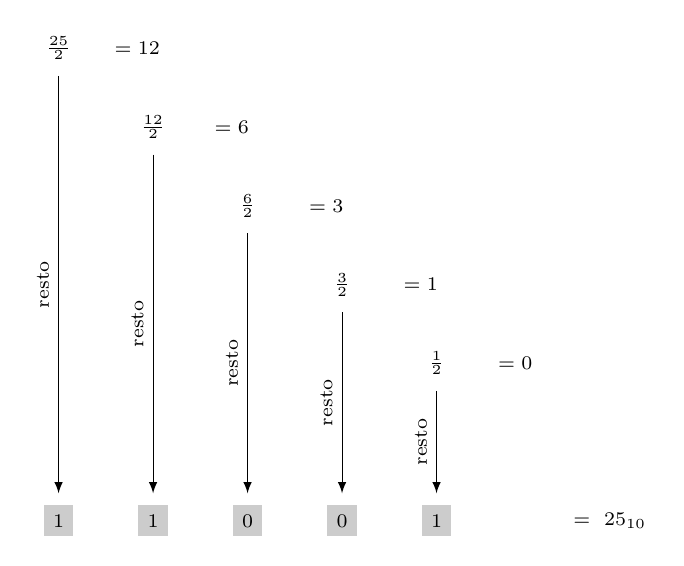
\begin{tikzpicture}

  \tikzset{res/.style={fill=gray!40}}
  \foreach \i/\num/\res/\rest in {0/25/12/1,1/12/6/1,2/6/3/0,3/3/1/0,4/1/0/1} {
    \node at (1.2*\i,-\i) {${\num\over 2}$};
    \node at (1+1.2*\i,-\i) {${=\res}$};
    \node[fill=gray!40] at (1.2*\i,-6) {${\rest}$};
    \path[->,draw,>=latex] (1.2*\i,-\i-0.35) -- node[rotate=90,above]{resto}  (1.2*\i,-5.65);
}
\node at (7,-6) {$=\ 25_{10}$};
\end{tikzpicture}


  \label{fig:dec2bin}
  \caption{Método de conversão de decimal para binário utilizando divisões
    sucessivas.}
\end{figure}

 %%%%%%%%%%%%%%%%%%%%%%%%%%%%%%%% SEC:HEX

\subsection[sec:num:hex]{Sistema de numeração hexadecimal}


\begin{enumerate}
\item Conversão de decimal em hexa;
\item Conversão de hexa em binário;
\item Conversão de binário em hexa;
\item Contagem em hexadecimal;
\item Vantagens do sistema hexa.
\end{enumerate}


\section{Circuitos Lógicos}
\label{ch:log-circ}


\subsection{Portas Lógicas}
\label{sec:gates}

\def\ltruthtable{ e correspondente tabela-verdade}

\begin{figure}[ht]
  \centering
  
%%% Local Variables:
%%% mode: latex
%%% End:

\begin{tikzpicture}  

    \node[or gate US, minimum height=2cm, draw] at (-6,0) (G) {};
    \draw (G.input 1 -| -8,0) node[anchor=east] {$i$} -- (G.input 1); 
    \draw (G.input 2 -| -8,0) node[anchor=east] {$c$} -- (G.input 2); 
    \draw (G.output) -- ([xshift=0.5cm]G.output) node[anchor=west] {$x$};

    \def\OR{{\tt OR}}


    \matrix (or truth table) [matrix of nodes]
    {\hline
      $i$ & $c$ & $x$ \\\hline
      0 & 0 & 0 \\
      0 & 1 & 1 \\
      1 & 0 & 1 \\
      1 & 1 & 1 \\
    };

\end{tikzpicture}

  \caption{Porta Lógica OR \ltruthtable.}
  \label{fig:or:gate}
\end{figure}

\begin{figure}[ht]
  \centering
  \input{\imgdir/and-gate}
  \caption{Porta Lógica AND \ltruthtable.}
  \label{fig:and:gate}
\end{figure}

\begin{figure}[ht]
  \centering
  
%%% Local Variables:
%%% mode: latex
%%% End:

\begin{tikzpicture}
\node[not gate US, minimum height=2cm, draw] at (-6,0) (G) {};
\draw (G.input -| -8,0) node[anchor=east] {$i$} -- (G.input); 
\draw (G.output) -- ([xshift=0.5cm]G.output) node[anchor=west] {$x$};

\def\NOT{{\tt NOT}}
\matrix (not truth table) [matrix of nodes]
{\hline
  $i$ & $x$ \\\hline
   0 &  1 \\
   1 &  0 \\
};

\end{tikzpicture}
  


  \caption{Porta Lógica NOT \ltruthtable.}
  \label{fig:not:gate}
\end{figure}
          
\begin{figure}[ht]
  \centering
  
%%% Local Variables:
%%% mode: latex
%%% End:

\begin{tikzpicture}
\def\XOR{{\tt XOR}}

\node[xor gate US, minimum height=2cm, draw] at (-6,0) (G) {};
\draw (G.input 1 -| -8,0) node[anchor=east] {$i$} -- (G.input 1); 
\draw (G.input 2 -| -8,0) node[anchor=east] {$c$} -- (G.input 2); 
\draw (G.output) -- ([xshift=0.5cm]G.output) node[anchor=west] {$o$};

\matrix (xor truth) [matrix of nodes]
{\hline
  $i$ & $c$ & $o$\\\hline
  0 & 0 & 0 \\
  0 & 1 & 1 \\
  1 & 0 & 1 \\
  1 & 1 & 0 \\
};

\end{tikzpicture}

  \label{fig:xor:gate}
  \caption{Porta Lógica XOR \ltruthtable.}
\end{figure}


\subsection{Lógica Combinacional}

\subsubsection{Noções de Álgebra Booleana}

As operações sobre $0$s e $1$s são chamadas operações booleanas em
homenagem a George Boole, que em seu livro ``A Investigation of the
Laws of Thought'' escrito em 1854, confinou as operações aritméticas
ordinárias sobre $0$s e $1$s.

% TODO ler o livro e colocar um formula sua
Apesar de Boole ter utilizado operadores aritméticos ($x+(1-x)$) para demonstrar
as leis, ele garantia que o resultado de uma disjunção nunca fosse
igual a $2$.

Utilizando a notação moderna, usamos a seguinte notação para
representar as operações booleanas:

\begin{table}[ht]
  \centering
  \begin{tabular}{c|c|c}\hline
  \bf Notações &\bf Operador &\bf Nome \\\hline
  $xy, x\land y$, $x$ \& $y$ & $\land$ & conjunção \\
  $x\lor y, x|y$ & $\lor$ & disjunção \\
  $\lcompl{x}, \lnot x, !x, \sim x$ & $\lnot$ & negação \\
  $x\lxor y, x\not\equiv y,x\hat y$ & $\lor$ &
  disjunção exclusiva, {\em xor}\\\hline
\end{tabular}

\label{tab:bool:op}
\caption{Algumas operações lógicas da álgebra booleana.}
\end{table}

Dentre algumas propriedades compartilhada pela álgebra booleana, a lei
distributiva é uma delas, portanto:


\begin{equation}
   (x\lor y) \land z = (x\land z)\lor (y\land z)
   \label{eq:distor}
\end{equation}

\begin{equation}
  (x\land y) \lor z = (x\lor z)\land (y\lor z)
  \label{eq:distand}
\end{equation}



\topic{Identidades básicas.} Os quatro operadores fundamentais da
álgebra booleana, $\land, \lor, \lxor, \lcompl{\ }$ podem expressar
outras operações. Cada um dos $\land, \lor, \lxor$ é associativo e
comutativo, além das leis distributivas de $\in{(}{)}$[eq:distor] e
$\in{(}{)}$[eq:distand] temos

\begin{equation}
  (x\lxor y) \land z = (x\land z) \lxor (y \land z),
\label{eq:distributive}
\end{equation}

\noindent bem como as {\em leis de absorção}

\begin{equation}
  (x\land y) \lor x = (x\lor y) \land x = x.
  \label{eq:xor:absorption}
\end{equation}

\noindent Uma das identidades mais simples e úteis é

\begin{equation}
x \lxor x = 0,
  \label{eq:xor:identity}
\end{equation}

\noindent pois isto implica, entre outras coisas

\begin{equation}
  (x\lxor y) \lxor x = y, \quad (x\lxor y) \lxor y = x.
  \label{eq:xor:absorption2}
\end{equation}

Em outras palavras, dado $x\lxor y$ e $x$ ou $y$, é fácil determinar o
outro. Além disso, a {\em lei do complementação}

\begin{equation}
  \lcompl{x} =  x \lxor  1.
  \label{eq:complementation}
\end{equation}


\topic{Leis de Morgan.} Augustus de Morgan enunciou em 1858 as
seguintes leis, hoje conhecidas como Leis de Morgan:

\begin{equation}
  \lcompl{x\land y} = \lcompl{x} \lor \lcompl{y}  
  \label{eq:morgan:and}
\end{equation}

\begin{equation}
\lcompl{x\lor y} = \lcompl{x} \land \lcompl{y}  
\label{eq:morgan:or}
\end{equation}

\exercise~Desenhar o esquema de circuito e a tabela verdade para as
seguintes expressões booleanas:

\begin{enumerate}
\item $u = (x \land y) \lor z$
\item $u = (x \lor y) \land z$
\end{enumerate}
  
\subsubsection{Multiplexador}
\begin{figure}[ht]
  \centering
  \begin{tikzpicture}
  
\def\shift{1cm}
\begin{scope}
  \tikzset{every node/.style={font=\scriptsize},
   every path/.style={->,>=latex, draw},
    mux/.style={rotate=90, minimum height=.5*\shift,minimum width=2*\shift, rounded
      corners=2mm, draw},
    l/.style={gray}
}

    \node[mux] (MUX) at (0,0) {};
    \node[l] (M) at ([yshift=.25*\shift]MUX) {m};
    \node[l] (u) [below of=M,yshift=.75\shift] {u};
    \node[l] (x) [below of=u,yshift=.75\shift] {x};

    \node at ([xshift=-1.5*\shift]MUX.20) (A) {x};
  
    \path  (A) -- (MUX.20) node[right,xshift=1] {$0$};

    \node (B) at ([xshift=-1.5*\shift]MUX.160) {y};
  
    \path (B) -- (MUX.160) node[right,xshift=1] {$1$};

    \node (C) at ([xshift=1.5*\shift]MUX.south) {f};
  
    \path  (MUX.south) -> (C);
  
    \node (S) at ([yshift=-1.5*\shift]MUX.west) {seleção $s$};
  
    \path[->,>=latex]  (S) -> (MUX.west);

    

   \matrix (select table) [matrix of nodes, above of=MUX,xshift=-.5\shift,yshift=\shift]
   {
     \bf s & \bf f \\
     0 & =x \\
     1 & =y \\
   };

\end{scope}

\begin{scope}

  %GATES
  \draw
  (5,1) node[and gate US,draw] (andA){}
  (5,-1) node[and gate US,draw] (andB){}
  (7,0) node[or gate US,draw] (orC){}
  (andA.output) -| (orC.input 1)
  (andB.output) -| (orC.input 2);
  \node[above] (LC) at (orC.output) {$f$};

  %+WIRE
  \path[draw] (andA.input 1) node[] (anchor A) {} -- +(-.5,0) node[above] {x};
  \path[draw] (andB.input 2) node[] (anchor B) {} -- +(-.5,0) node[above] {y};

  \node[] at (andA.input 2) (wire inAtwo)  {};
  \node[ocirc] [right of=wire inAtwo,xshift=-.8*\shift] {};

  % SIGNAL
  \node[right] (S) [below of=anchor B] {seleção $s$};
  \path[draw] (S) -- (andB.input 1) node[circ] {} -- (andA.input 2);

   \node[green!30!black] (EXP) [below of=orC,xshift=.125*\shift,yshift=-\shift] {$f~(s,x,y) = x\overline{s} + ys$};
   

  \end{scope}
  
\end{tikzpicture}

  \label{fig:mux:symbol}
  \caption{Esquema de um multiplexador (seletor) de 1 bit.}
\end{figure}

\begin{figure}[ht]
  \centering
  \begin{tikzpicture}
  
\def\shift{1cm}
\begin{scope}
  \tikzset{every node/.style={font=\scriptsize},
   every path/.style={->,>=latex, draw},
    mux/.style={rotate=90, minimum height=.5*\shift,minimum width=2*\shift, rounded
      corners=2mm, draw},
    l/.style={gray}
}

    \node[mux] (MUX) at (0,0) {};
    \node[l] (M) at ([yshift=.25*\shift]MUX) {m};
    \node[l] (u) [below of=M,yshift=.75\shift] {u};
    \node[l] (x) [below of=u,yshift=.75\shift] {x};

    \node at ([xshift=-1.5*\shift]MUX.20) (A) {x};
  
    \path  (A) -- (MUX.20) node[right,xshift=1] {$0$};

    \node (B) at ([xshift=-1.5*\shift]MUX.160) {y};
  
    \path (B) -- (MUX.160) node[right,xshift=1] {$1$};

    \node (C) at ([xshift=1.5*\shift]MUX.south) {f};
  
    \path  (MUX.south) -> (C);
  
    \node (S) at ([yshift=-1.5*\shift]MUX.west) {seleção $s$};
  
    \path[->,>=latex]  (S) -> (MUX.west);

    

   \matrix (select table) [matrix of nodes, above of=MUX,xshift=-.5\shift,yshift=\shift]
   {
     \bf s & \bf f \\
     0 & =x \\
     1 & =y \\
   };

\end{scope}

\begin{scope}

  %GATES
  \draw
  (5,1) node[and gate US,draw] (andA){}
  (5,-1) node[and gate US,draw] (andB){}
  (7,0) node[or gate US,draw] (orC){}
  (andA.output) -| (orC.input 1)
  (andB.output) -| (orC.input 2);
  \node[above] (LC) at (orC.output) {$f$};

  %+WIRE
  \path[draw] (andA.input 1) node[] (anchor A) {} -- +(-.5,0) node[above] {x};
  \path[draw] (andB.input 2) node[] (anchor B) {} -- +(-.5,0) node[above] {y};

  \node[] at (andA.input 2) (wire inAtwo)  {};
  \node[ocirc] [right of=wire inAtwo,xshift=-.8*\shift] {};

  % SIGNAL
  \node[right] (S) [below of=anchor B] {seleção $s$};
  \path[draw] (S) -- (andB.input 1) node[circ] {} -- (andA.input 2);

   \node[green!30!black] (EXP) [below of=orC,xshift=.125*\shift,yshift=-\shift] {$f~(s,x,y) = x\overline{s} + ys$};
   

  \end{scope}
  
\end{tikzpicture}

  \label{fig:mux:gate}
  \caption{Possível combinação de portas lógicas para um multiplexador
    (seletor) de 1 bit.}
\end{figure}

\bibliographystyle{plain}
\bibliography{digisys}

\end{document}
           
